%=========================================
% 	   Fallstudie     		 =
%=========================================
\chapter{Fallstudie}
\label{ch:fallstudie}
In den vorherigen Kapiteln wurde auf das Architekturmuster Cloud-Native und dessen Eigenschaften eingegangen. Ferner wurden Technologien vorgestellt, welche bei der Umsetzung einer Cloud-Native-Architektur unterstützen. In diesem Kapitel wird eine Fallstudie betrachtet, welche eine naive Umsetzung der Cloud-Native-Architektur anhand eines beispielhaften Softwareprojektes darstellt. Diese soll im Anschluss evaluiert werden.

\section{Vorstellung der Fallstudie}

Um das Thema "Cloud-Native-Architekturen" innerhalb eines Beispielprojektes darzustellen, wurden zunächst verschiedene Ideen evaluiert. Zu ihnen gehörten unter anderem ein kleiner Webshop, ein Videokommunkationsservice über WebRTC und ein soziales Netzwerk zum Teilen von Bildern. Schlussendlich fiel die Wahl auf ein Minimalbeispiel für eine  Online-Wahlplatform. In der Realität müssten eine solche Wahlplatform ihre Komponenten bei einer großen Menge von Anfragen in der Lage sein, entsprechend zu skalieren. TODO:blablabla

\section{Anforderungen}

Die Anforderungen an die Fallstudie können in funktionale und nicht funktionale Anforderungen eingeteilt werden. Funktionale Anforderungen beschreiben diejenigen Anforderungen, die zur Funktion des Softwareprojektes unbedingt nötig sind. Nichtfunktionale Anwendungen legen alle Randbedingungen fest, die zur Qualität der Ausführung der Software adressiert und umgesetzt werden müssen und über die funktionalen Anforderungen hinaus gehen [quelle: Chris Rupp: Requirements-Engineering und -Management: Aus der Praxis von klassisch bis agil]. 

\subsection{Funktionale Anforderungen}

Das durch die Fallstudie entstehende Softwareprojekt hat die Hauptaufgabe, ein Umfrage- oder Wahlgeschehen zu simulieren. Nutzer sollen in der Lage sein, über eine Webseite einen aus mehreren Kandidaten auszuwählen und abschließend für ihn eine Stimme abzugeben. Dabei geben sie nicht nur einen Kandidaten, sondern auch ihr Ursprungsland an. In der Praxis könnten diese Angaben noch um weitere Punkte erweitert werden.
Weiterhin soll es ihnen möglich sein, die Wahlergebnisse auf einer weiteren Web-Anwendung in Echtzeit zu verfolgen. Das Einsehen von Ergebnissen erfolgt hierbei sowohl nach der Anzahl der Stimmen für einen Kandidaten, als auch nach den Ergebnissen für einen Kandidaten pro Abstimmungsort. Zur leichteren Einsicht sollen die Ergebnisse auf letzterer Web-Anwendung graphisch dargestellt werden. 

\subsection{Nichtfunktionale Anforderungen}
Um einige, ausgewählte Anforderungen an eine Cloud-Native-Architektur beispielhaft darzustellen, sollen zur Umsetzung der Fallstudie entsprechende Technologien gewählt werden. Konkret soll die dabei Fallstudie die Kriterien \textit{Skalierbarkeit}, \textit{Modularität} und \textit{Erweiterbarkeit} erfüllen. 

\section{Konzeption}
Um unsere Wahl-Applikation zu realisieren, müssen die einzelnen Funktionalitäten zunächst in eigene Mikroservices aufgeteilt werden. Wir haben uns dafür entschieden, fünf bzw. mit Datenbank sechs Microservices zu verwenden.
\\\\
Die ersten beiden Microservices stellen das Userinterface unserer Anwendung dar. Es gibt jeweils einen Microservice für das Voting-Frontend (\lstinline{frontend-voting}), über welches eine Stimme abgegeben werden kann, sowie einen Microservice für das Analysis-Frontend (\lstinline{frontend-analysis}), welches das aktuelle Ergebnis der Wahl visualisiert.
\\\\
Es gibt einen weiteren Microservice \lstinline{service-raw-data}, welcher für das Speichern und Abrufen von Daten verantwortlich ist. Dieser ist mit einer Datenbank verbunden, in unserem Fall einer Redis-Datenbank. Er bietet zwei Funktionalitäten an: das Speichern einer neu abgegebenen Stimme und das Ausgeben aller bisher erhaltenen Stimmen. Um die Stimmen nun zu aggregieren, also beispielsweise die Stimmen für ein Land ausgeben zu lassen, wird ein eigener Microservice \lstinline{service-calculate} verwendet, welcher für Berechnungen auf den bisher abgegebenen Stimmen zuständig ist. Er erhält die aktuellen Daten vom \lstinline{service-raw-data}.
\\\\
Wir haben außerdem noch einen weiteren Microservice \lstinline{service-serving-layer} eingeführt, welcher für die Kommunikation zwischen den einzelnen Microservices zuständig ist. Er bildet somit eine einheitliche Schnittstelle für das Frontend zum \dq Backend\dq\,unserer Anwendung und koordiniert die einzelnen Anfragen zwischen den einzelnen Microservices.
\\\\
Unsere Anwendung besteht somit aus den folgenden Komponenten:
\\\\
\begin{figure}[bth]
  \centering
  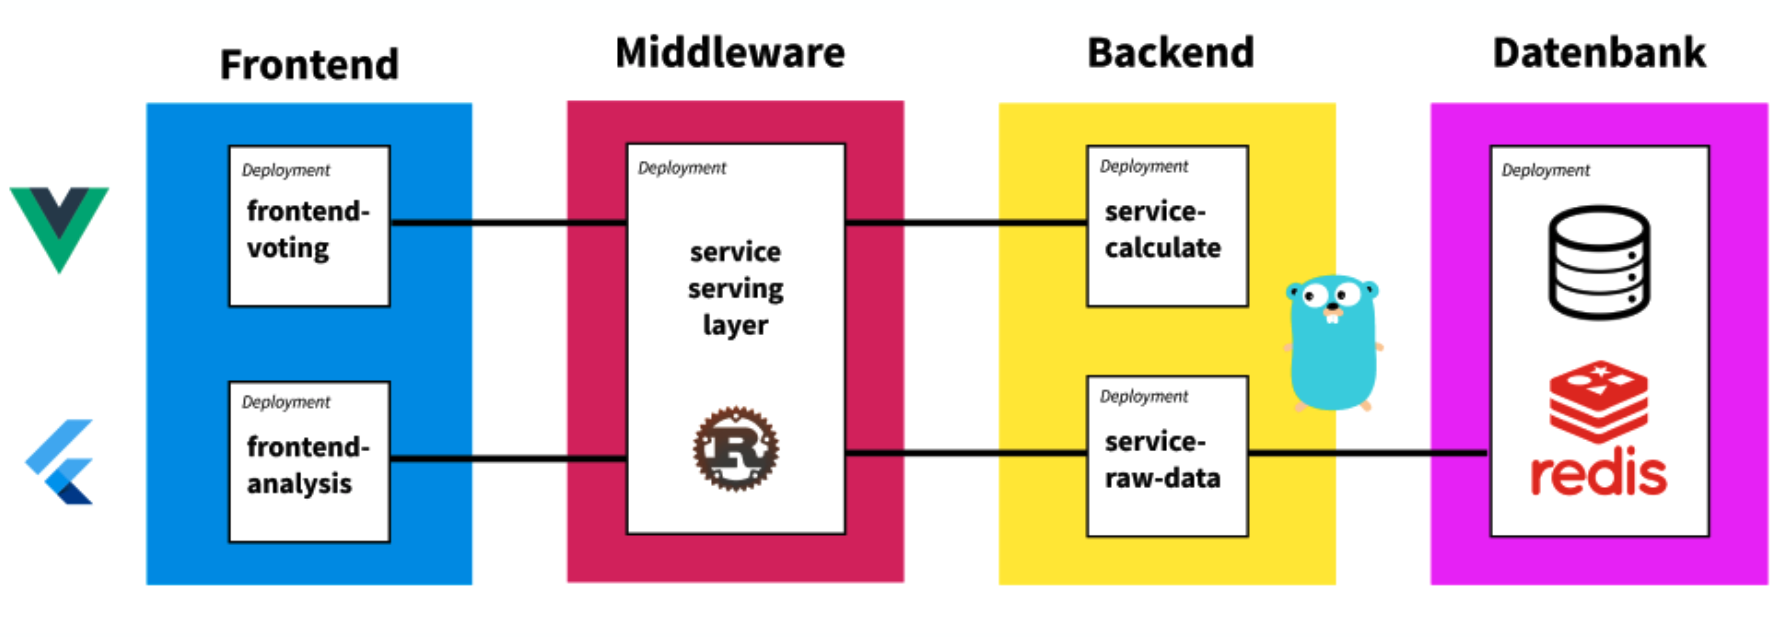
\includegraphics[width=0.9\textwidth]{Chapters/5-Fallstudie/Graphics/SA-Architektur.png}
  \caption{Architektur Microservices}
  \label{fig:architecture}
\end{figure}
\\\\
Wir haben uns für diese Architektur entschieden, da somit jeder Microservice abgesehen von der Datenbank stateless ist. Somit können alle Microservices beliebig skaliert werden.\\\\
Wenn nun eine Stimme abgegeben wird, wird von \lstinline{frontend-voting} die Stimme zu 
\lstinline{service-serving-layer} gesendet, welcher sie weiter an \lstinline{service-raw-data} reicht, welcher sie dann anschließend in der Datenbank speichert.\\
Wird ein Ergebnis der Wahl abgefragt, so sendet \lstinline{frontend-analysis} diese Anfrage zu \lstinline{service-serving-layer}, welcher die Anfrage zu \lstinline{service-calculate} weiter reicht. Dieser benötigt nun alle bisher abgegebenen Stimmen, um ein Ergebnis zu berechnen. Hierfür frägt er wiederum \lstinline{service-serving-layer} an, welcher die Anfrage an \lstinline{service-raw-data} weiter reicht. Dieser gibt alle bisher abgegebenen Stimmen zurück, anhand derer \lstinline{service-calculate} dann das Ergebnis berechnet und zurück gibt.

\section{Umsetzung}
Da die einzelnen Microservices voneinander unabhängig sind, und in der Praxis oft von unterschiedlichen Teams entwickelt werden, haben wir uns um dies zu veranschaulichen dafür entschieden, für unsere Microservices verschiedene Programmiersprachen zu verwenden.
\\\\
Für den Service \lstinline{frontend-voting} wurde das JavaScript Framework Vue.js verwendet, während \lstinline{frontend-analysis} in Dart geschrieben ist. Für \lstinline{service-serving-layer} wurde die Programmiersprache Rust eingesetzt. Die beiden anderen Services, \lstinline{service-raw-data} und \lstinline{service-calculate} sind beide in Go geschrieben.
\\\\
Für das Erstellen unserer Container-Images haben wir Docker verwendet, da es sich hierbei um das bekannteste Tool in diesem Bereich handelt und es mit Hilfe von Dockerfiles eine sehr einfache Möglichkeit bietet, Container-Images zu erstellen. Außerdem haben wir DockerHub für das Austauschen unserer Images eingesetzt.
\\\\
Als Container-Orchestrator haben wir Kubernetes eingesetzt. Da wir kein Cluster mit mehreren Nodes zur Verfügung hatten, um unsere Anwendung zu deployen, haben wir hierfür Minikube verwendet. Minikube bietet die Möglichkeit, ein Kubernetes-Cluster mit einem einzigen Node innerhalb einer VM aufzusetzen \cite{noauthor_minikube_2021}. Es ist somit gut dafür geeignet, Cloud-Native-Anwendungen lokal auf einem Rechner auszuführen und zu testen.
\\\\
Jeder unserer Stateless-Microservices wird in Kubernetes als einzelnes Deployment abgebildet und kann somit beliebig oft dupliziert werden. Dadurch können die einzelnen Microservices beliebig skaliert werden. Dies trifft jedoch nicht auf unsere Datenbank zu. Wir haben uns der ansonsten stark erhöhten Komplexität dafür entschieden, unsere Datenbank nicht skalierbar sowie nicht persistent zu machen. Es existiert somit immer nur ein Pod unserer Datenbank und diese kann in unserem Fallbeispiel nicht skaliert werden. 
\section{Evaluation}
Abschließend gilt es zu betrachten, auf welche Probleme wir während der Umsetzung gestoßen sind. Hier muss angemerkt werden, dass die Umsetzung in einem engen Zeitrahmen statt gefunden hat. Jedes der gezeigten Konzepte kann noch weiter ausgearbeitet werden. Ferner wird jedes der gezeigten Konzepte exponentiell komplexer, sollte die Anwendung in einer produktiven Umgebung eingesetzt werden. Einige dieser Konzepte werden in den folgenden Abschnitten erläutert. Zunächst gilt es allerdings zu analysieren, was unsere Anwendung bereits im aktuellen Zustand problemlos umsetzen kann.\\
\\
Im Kapitel Konzeption wurden die einzelnen Komponenten unser Anwendung gezeigt. Jede dieser Komponenten stellt ein eigenes Kubernetes Deployment dar. Dies ermöglicht es jede dieser Komponenten zu skalieren. Die Kommunikation der Komponenten untereinander ist weiterhin problemlos möglich. Ferner werden Nutzeranfragen auf die verschiedenen Instanzen der Benutzerschnittstellen verteilt. Von außen ist nicht ersichtlich, dass mehrere Instanzen der Komponenten betrieben werden. Unsere Anwendung könnte demnach auf einem Kubernetes Cluster betrieben werden. Stellt dieses genügen Rechen-Ressourcen bereit kann eine beliebige Anzahl an Nutzern die Anwendung nutzen. Hierbei ergeben sich Einschränkungen und Probleme. Diese werden in den nächsten Abschnitten näher beleuchtet.
\subsection{Umgang mit State}
Im Kapitel Konzeption wurde bereits klar, dass der \lstinline{calculate-service} stets den \lstinline{serving-layer-service} nutzt um den \lstinline{raw-data-service}, und damit die Datenbank, zu kontaktieren. Der \lstinline{calculate-service} verwaltet keine Art von Cache. Dies ist Teil der Bemühung die Komponenten weitestgehend stateless zu halten. Eine Skalierung von stateless Komponenten ist problemlos möglich. Die einzelnen Instanzen müssen in diesem Fall keine Informationen untereinander teilen und  konsistent halten. Letzteres reduziert die Komplexität der Anwendung. Um dennoch stateful Deployments anzulegen stellt Kubernetes Konzepte wie \textit{Stateful-Sets} \cite{noauthor_statefulsets_nodate} zur Verfügung. Im Rahmen dieser Fallstudie wurden\textit{ Stateful-Sets} nicht betrachtet. 
\subsection{Die Datenbank}
Im Rahmen dieser Umsetzung wurde eine Redis Datenbank verwendet. Diese ist von Natur aus stateful. Im vorherigen Abschnitt wurde bereits erläutert, warum dies eine Herausforderung darstellt. Im Rahmen unserer Fallstudie wird die Datenbank nicht skaliert. Sie befindet sich in einem einzigen Deployment mit einem einzigen Pod. Dies ist natürlich in einem produktiv Environment nicht praktikabel. \\
Unserer Umsetzung kann als Abwandlung eines Shared-Repositorys gesehen werden. Der \lstinline{raw-data-service} stellt dabei das Shared-Repository da. Der Redis-Pod den persistenten Speicher. Ein Nachteil dieses Vorgehens ist die fehlende Skalierbarkeit und die Datenbank als Single-Point-of-Failure.\\
Redis bietet allerdings ein Master/Slave Modell an. Dieses nutzt sogenannte Hash-Slots. Jede der Redis Instanzen verwaltet dabei eine abgeschlossene Menge dieser Hash-Slots. Die Daten werden also effektiv unter den Redis-Instanzen verteilt. In der Umsetzung der Fallstudie wurde dieses Konzept nicht genutzt. \cite{noauthor_redis_nodate} \\
Darüber hinaus muss angemerkt werden, dass die Datenbank auch nicht persistiert wird. Ein Neustart des Clusters führt zur Erstellung neuer Pods. Folglich wird auch eine neue Instanz der Datenbank angelegt. Auch hierfür wären Stateful-Sets \cite{noauthor_statefulsets_nodate} ein Lösungsansatz. 
\subsection{Kommunikations-Logik}
Jeder der Micro-Services geht davon aus, dass die jeweils anderen Micro-Services erreichbar sind. Dabei wurde nur minimales Error-Handling umgesetzt. In einer Produktiv-Umgebung gilt es unter anderem eine zentrale Retry-Logik umzusetzen.\\
Ferner wird die Kommunikation nicht abgesichert. Jede Kommunikation innerhalb des Clusters und außerhalb des Clusters findet über reines HTTP statt. Ein mitlesen der Kommunikation ist damit problemlos möglich.\\
Darüber hinaus kann jeder Micro-Service die Kommunikation der anderen Micro-Services einsehen. Um diese Probleme zu lösen eignet sich ein Service-Mesh, wie zum Beispiel Istio \cite{istio_istio_nodate}.
















